\documentclass{beamer}
\usetheme{Madrid}

\usepackage{amsmath, amssymb, amsthm}
\usepackage{graphicx}
\usepackage{listings}
\usepackage{gensymb}
\usepackage{minted}
\usemintedstyle{friendly}
\definecolor{bg}{rgb}{0.95,0.95,0.95}
\usepackage[utf8]{inputenc}
\usepackage{hyperref}
\usepackage{gvv}\begin{document}
\title{12-9-6-2}
\author{EE23BTECH11060 - SRUTHI BIJILI $^{*}$}
\date{}
\frame{\titlepage}

\begin{frame}
\frametitle{Question}
Find the general equation of 
\begin{align}
    \frac{dy}{dx}+3y=e^{-2x}
\end{align}
\end{frame}
\begin{frame}{allowframebreaks}
\frametitle{Theoretical solution}
Laplace transform of the derivative $\frac{dy}{dx}$ is given by 
\begin{align}
    \mathcal{L}\cbrak{\frac{dy}{dx}}=sY\brak{s}-y\brak{0}
\end{align}
where Y\brak{s} is the laplace transform of y\brak{x},and y\brak{0} is the initial condition.\\
taking laplace transform on both sides of the equation:
\begin{align}
    \mathcal{L}\cbrak{\frac{dy}{dx}+3y}=\mathcal{L}\cbrak{e^{-2x}}\\
    \implies \mathcal{L}\cbrak{\frac{dy}{dx}}+\mathcal{L}\cbrak{y}=\mathcal{L}\cbrak{e^{-2x}}\\
    \mathcal{L}\cbrak{e^{-2x}}=\frac{1}{s+2}\\
    \implies sY\brak{s}-y\brak{0}+3Y\brak{s}=\frac{1}{s+2}
\end{align}
\end{frame}
\begin{frame}
\frametitle{Theoretical solution}
rearranging the equation 
\begin{align}
    Y\brak{s}=\frac{1}{\brak{s+2}\brak{s+3}}+\frac{y\brak{0}}{s+3}\\
     Y\brak{s}=\frac{1}{\brak{s+2}}-\frac{1}{\brak{s+3}}+\frac{y\brak{0}}{s+3}
\end{align}
Taking the inverse laplace transform of each term:
\begin{align}
    \mathcal{L}^{-1}\cbrak{Y\brak{s}}=\mathcal{L}^{-1}\cbrak{\frac{1}{s+2}}+\mathcal{L}^{-1}\cbrak{\frac{1}{s+3}}
\end{align}
thus,the solution by laplace transform is 
\begin{align}
    y\brak{x}=e^{-2x}-e^{-3x}+y\brak{0}e^{-3x}\\
    \implies  y\brak{x}=e^{-2x}+\brak{y\brak{0}-1}e^{-3x}\\
\end{align}
\end{frame}
\begin{frame}[fragile]
\frametitle{Method of finite differences}
The derivative of f(x) can be written as 
\begin{align}
    \frac{df}{dx}=\frac{f(x+h)-f(x)}{h}\\
    \implies f(x+h)=f(x)+h\cdot\frac{df}{dx}
\end{align}
from the above question 
\begin{align}
    \frac{dy}{dx}+3y=e^{-2x}\\
    \implies \frac{dy}{dx}=e^{-2x}-3y\\
    \implies y(x+h)=y(x)+h\brak{e^{-2x}-3y}
\end{align}
for $x \in \sbrak{x_{0},x_{n}}$ divide into equal parts by difference h\\
Let us assume that $x_{0}=0$,$y_{0}=1$\\
Let $x_{1}$=$x_{0}+h$ then
\begin{align}
    y_{1}=y_{0}+h\brak{e^{-2x_{0}}-3y_{0}}
\end{align}
\end{frame}
\begin{frame}[fragile]
\frametitle{Method of finite differences}
To obtain the graph repeat the process until sufficient points to plot the graph and the general equation will be 
\begin{align}
    x_{n+1}=x_{n}+h\\
    y_{n+1}=y_{n}+h\brak{e^{-2x_{n}}-3y_{n}}
\end{align}
The curve generalised using the method of finite differences for the given question taking $x_{0}=0$,$y_{0}=1$, $h=0.01$ and running iterations for 100 times
\end{frame}
\begin{frame}
\frametitle{Simulation}
\begin{figure}
    \centering
    \centering
   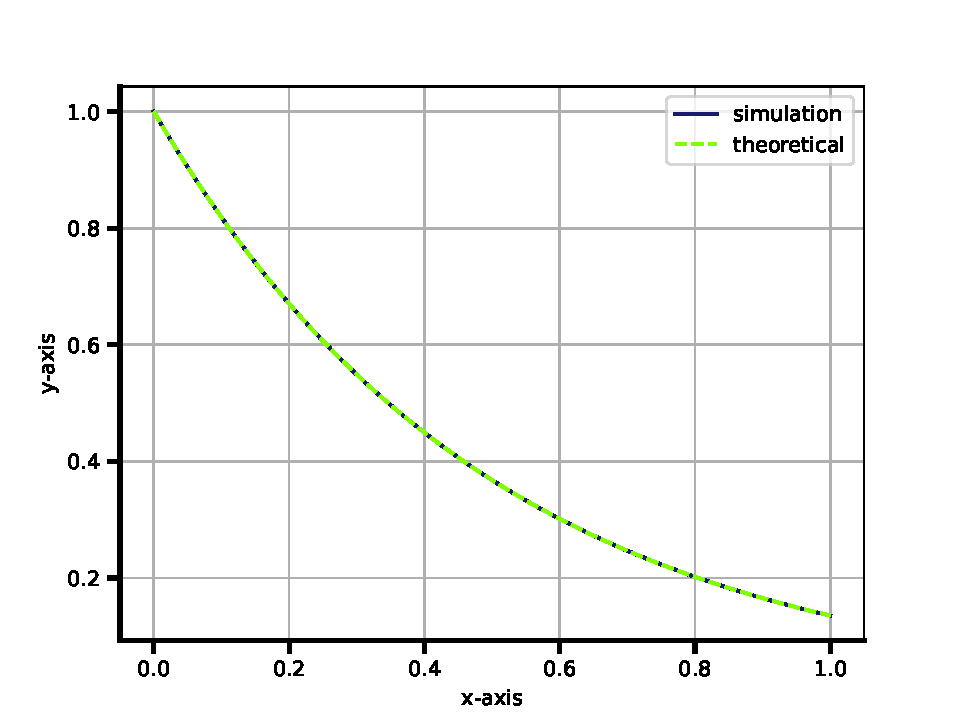
\includegraphics[width=0.7\columnwidth]{fig.pdf}
    \caption{}
    \label{fig:enter-label}
\end{figure}
\end{frame}
\begin{frame}[fragile]
\frametitle{C-Code}
\begin{minted}[bgcolor=bg, linenos, fontsize=\small, breaklines]{c}
#include<stdio.h>
#include<math.h>
double h=0.0002;
float dydx(float x, float y){
	return (-3*y+exp(-2*x));
}
void vals(float *x,float *y,int n){
	for(int i=0;i<n;i++){
		*y+=dydx(*x,*y)*h;
		*x+=h;
	}
}
\end{minted}
\end{frame}
\begin{frame}[fragile]
  \frametitle{Python Code }

\begin{minted}[bgcolor=bg, linenos, fontsize=\small, breaklines]{python}
import math
import ctypes
import matplotlib.pyplot as plt

# Loading the .so file
lib = ctypes.CDLL('./funcs.so')

# Definations of return types and argument types in C code
lib.vals.argtypes = [ctypes.POINTER(ctypes.c_float), ctypes.POINTER(ctypes.c_float), ctypes.c_int]
lib.vals.restype = None

lib.dydx.argtypes = [ctypes.c_float, ctypes.c_float]
lib.dydx.restype = ctypes.c_float

# Set the initial values and parameters
x = ctypes.c_float(0.0) 
y = ctypes.c_float(1.0)
\end{minted}
\end{frame}
\begin{frame}[fragile]
  frametitle{Python Code }

\begin{minted}[bgcolor=bg, linenos, fontsize=\small, breaklines]{python}
n = 5000
h = 0.0002
# Creating arrays to store the results for plotting
x_vals = []
y_vals = []
theory_values = []
# Generate values using the C function
for i in range(n):
    x_vals.append(float(x.value))
    y_vals.append(float(y.value))
# Compute theoretical values for y using the known solution of the ODE
    theory_y = math.exp(-2*x.value)
    theory_values.append(theory_y)  
    # Call the C function to update x and y
    lib.vals(ctypes.byref(x), ctypes.byref(y), 1)

\end{minted}
\end{frame}
\begin{frame}[fragile]
  \frametitle{Python Code }

\begin{minted}[bgcolor=bg, linenos, fontsize=\small, breaklines]{python}   
#plotting
sim_line, = plt.plot(x_vals, y_vals, label="simulation", color='midnightblue')
theory_line, = plt.plot(x_vals, theory_values, label="theoretical", color='chartreuse', linestyle='--')
plt.xlabel("x-axis")
plt.ylabel("y-axis")
# Customize axis spines for thick black axes
ax = plt.gca()  # Get the current axes
ax.spines['bottom'].set_color('black')  # Bottom axis
ax.spines['bottom'].set_linewidth(2)    # Set thickness
ax.spines['left'].set_color('black')    # Left axis
ax.spines['left'].set_linewidth(2)      # Set thickness
# Customize tick parameters for thicker black ticks
ax.tick_params(axis='both', colors='black', width=2, length=6)
plt.legend(handles=[sim_line, theory_line])
plt.grid(True)
plt.show()
\end{minted}
\end{frame}

\end{document}
\
